% Gemini theme
% https://github.com/anishathalye/gemini

\documentclass[20pt, final]{beamer}

% ====================
% Packages
% ====================

%\usepackage[T1]{fontenc}
\usepackage{lmodern}
\usepackage[size=a1, scale=1.0, orientation=portrait]{beamerposter}
\usetheme{gemini}
\usecolortheme{gemini}
\setbeamerfont{block body}{family=\Lato,size={\fontsize{18}{20}}}
\setbeamerfont{enumerate item}{size={\fontsize{18}{20}}}

\usepackage{graphicx}
\usepackage{booktabs}
\usepackage{tikz}
\usepackage{pgfplots}
\definecolor{amethyst}{rgb}{0.6, 0.33, 0.73}
\usepackage{fontawesome}
\pgfplotsset{compat=1.14}
\usepackage{anyfontsize}
\usepackage{tcolorbox}
\usepackage{wrapfig}
\usepackage{braket}
\usepackage{bm}


%% ---------- useful for the schema ---------

\usetikzlibrary{positioning,arrows,calc,math,angles,quotes}
\usetikzlibrary{arrows,automata}
\usetikzlibrary{positioning}
\usetikzlibrary{arrows.meta,
                bending,
                intersections,
                quotes,
                shapes.geometric}

\tikzset{
    state/.style={
           rectangle,
           rounded corners,
           draw=black, very thick,
           minimum height=1em,
           inner sep=2pt,
           text centered,
           },
}



\definecolor{darkmidnightblue}{rgb}{0.0, 0.2, 0.4}

% ====================
% Lengths
% ====================

% If you have N columns, choose \sepwidth and \colwidth such that
% (N+1)*\sepwidth + N*\colwidth = \paperwidth
\newlength{\sepwidth}
\newlength{\colwidth}
\setlength{\sepwidth}{0.025\paperwidth}
\setlength{\colwidth}{0.42\paperwidth}


% useful for the logos

\logoright{\includegraphics[height=4cm]{figures/qr-code.png}}
\logoleft{\includegraphics[height=4cm]{figures/qibo_qr.png}}

\newcommand{\separatorcolumn}{\begin{column}{\sepwidth}\end{column}}

% ====================
% Title
% ====================

\title{Density estimation via adiabatic quantum computing}

\author{Matteo Robbiati\inst{1  }\inst{2  }, Juan Manuel Cruz Martinez\inst{2  } and Stefano Carrazza\inst{1  }\inst{2  }\inst{3  }}


\institute[shortinst]{
  \inst{1  } TIF Lab, Dipartimento di Fisica, Universit\`a degli Studi
  di Milano, Milan, Italy. 

  \inst{2  } CERN, Theoretical Physics Department, CH-1211
  Geneva 23, Switzerland.

  \inst{3  } Quantum Research Center, Technology Innovation Institute, Abu Dhabi, UAE.
  }

% ====================
% Footer (optional)
% ====================

\footercontent{
  \includegraphics[height=2cm]{figures/qibo_logo.png} \qquad \qquad \qquad \,\,\,\,\,\,\,\, \qquad \quad
  
\includegraphics[height=2cm]{figures/unimi.png} \qquad \qquad \qquad \,\,\,\,\,\,\,\, \qquad \quad
  \includegraphics[height=2cm]{figures/infn.png} \qquad \qquad \qquad \,\,\,\,\,\,\,\, \qquad \quad
  \includegraphics[height=2cm]{figures/tii.png} \qquad \qquad \qquad \,\,\,\,\,\,\,\, \qquad \quad 
  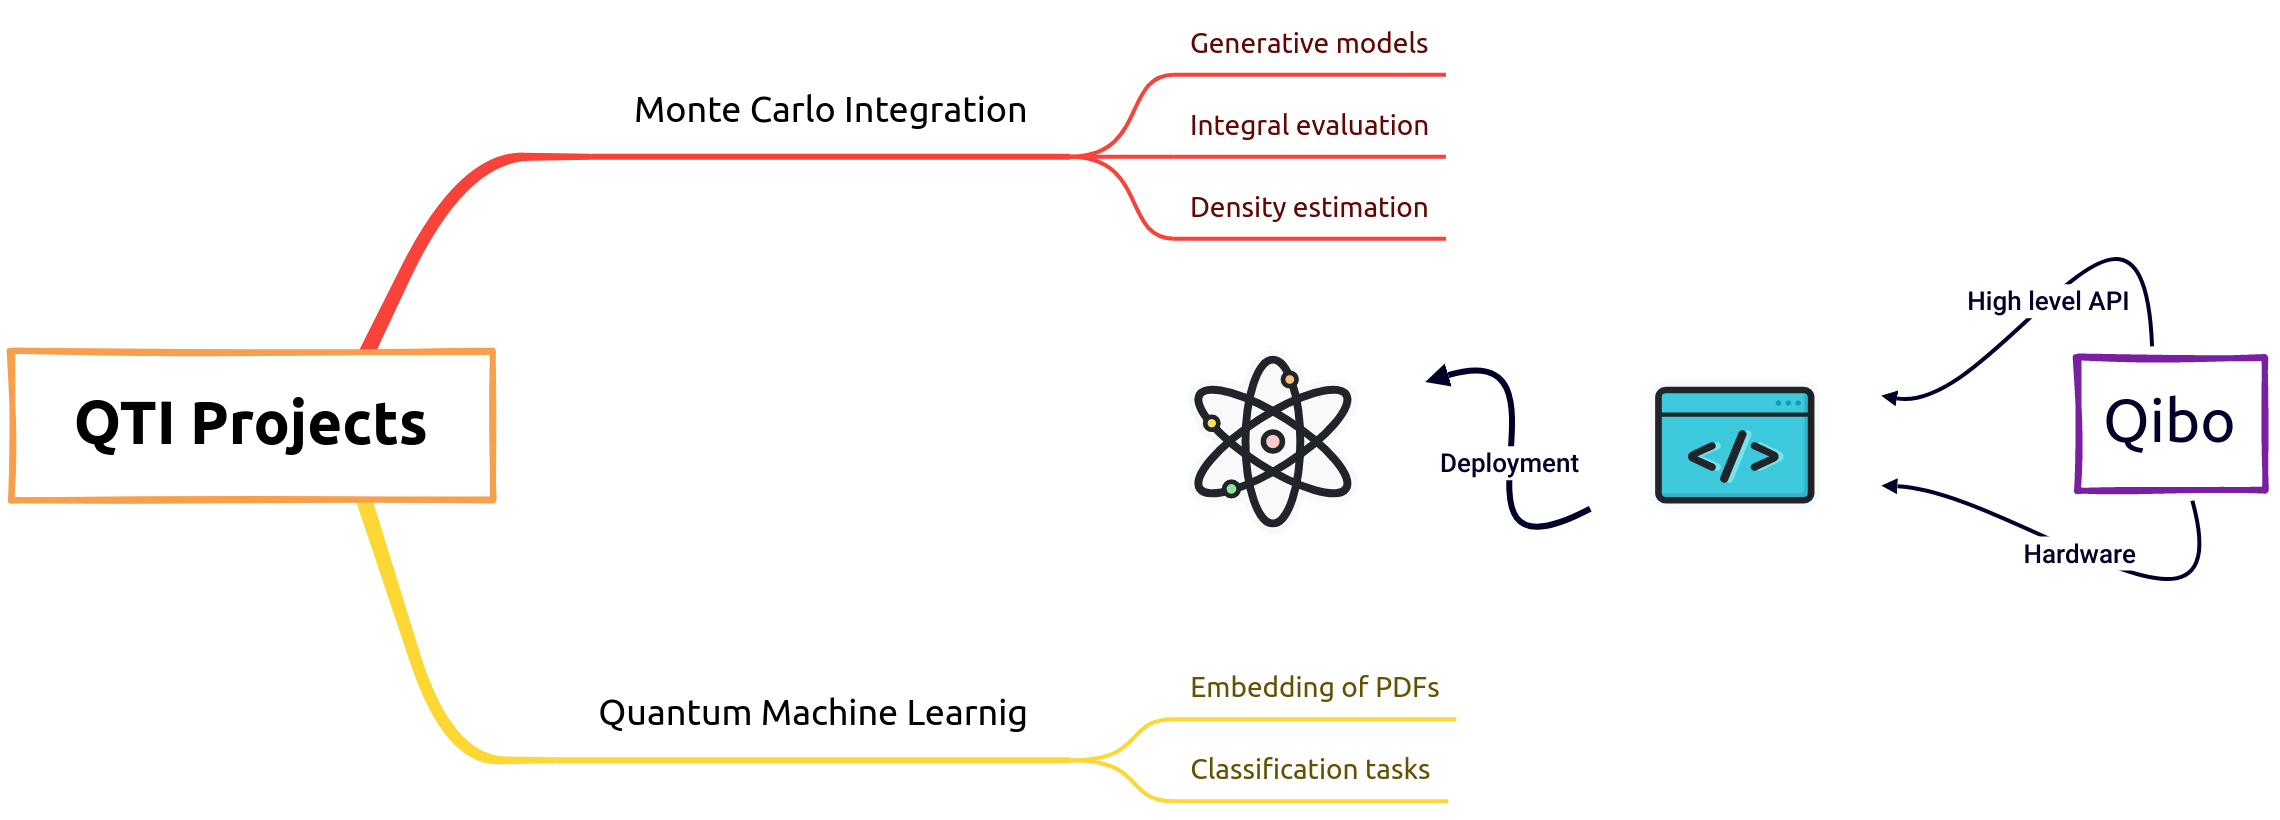
\includegraphics[height=2cm]{figures/qti.png} \qquad \qquad \qquad \,\,\,\,\,\,\,\, \qquad \quad
  \includegraphics[height=2cm]{figures/CERN.png} 
  \hfill
}
% (can be left out to remove footer)

% ====================
% Logo (optional)
% ====================

% use this to include logos on the left and/or right side of the header:
% \logoright{\includegraphics[height=7cm]{logo1.pdf}}
% \logoleft{\includegraphics[height=7cm]{logo2.pdf}}

% ====================
% Body
% ====================

\begin{document}

\begin{frame}[t]
\begin{columns}[t]
\separatorcolumn


\begin{column}{\colwidth}
\begin{alertblock}{Aim of the project}
We propose a novel strategy to perform density estimation: given a variable $\bm{x}$
sampled from an unknown distribution $\rho(\bm{x})$, we aim to 
estimate the puntual Probability Density Function (PDF) value $\hat{\rho}(\bm{x})$.

We focus on one-dimensional distributions, and then extend the 
study to the case of joint PDFs of indipendent variables.

% \faGamepad\,\, \textbf{Possible applications:} Monte Carlo Integration (MCI), Parton Distribution 
% determination, anomaly detection.

% To know the value of the probability of a given data $\bm{x}$ is important in many 
% situations, for example while calculating integrals via Monte Carlo Integration,
% where $\rho$ is used to correctly weight the sample points in the integral approximation.

\end{alertblock}
\begin{block}{Schematic pipeline of the algorithm}

  \begin{figure}
    \includegraphics[width=1  \textwidth]{figures/diagram.pdf}
  \end{figure}
\end{block}

\begin{block}{\faChain\,\, Encoding a CDF into an adiabatic evolution}
  
  We use \texttt{Qibo}~\cite{Efthymiou_2021} to simulate an adiabatic evolution on time $\tau$
  \begin{equation}
  H_{\rm ad}(\tau| \bm{\theta}) = \bigl[ 1 - s(\tau| \bm{\theta}) \bigr] H_0 + 
  s(\tau| \bm{\theta}) H_1 \ ,
  \end{equation}
Where $s(\tau | \bm{\theta})$ is a parametric scheduling function.

We map $\{x, F(x)\}$ into $\{\tau, -E(\tau)\}$ , where $E(\tau)$ energy of a 
non-interacting Pauli Z over the evolved ground state of $H_{\rm ad}$ at $\tau$.

\begin{figure}
    \includegraphics[width=0.65\textwidth]{figures/evolution.pdf}
\end{figure}
\end{block}

  \begin{alertblock}{Optimizing the adiabatic evolution}
  
  \begin{enumerate}
    \item perform the evolution with initial guess $\bm{\theta}_0$ in the scheduling;
    \item estimate a loss function $J_{\rm mse}\bigl[F, -E(\bm{\theta})\bigr]$;
    \item update $\bm{\theta}$ using a chosen optimizer until convergence.
  \end{enumerate}

  \end{alertblock}
  

  \begin{block}{\faPencil\,\, Building a derivable circuit}
  After encoding the CDF into the evolution, we translate $H_{\rm ad}$ into a circuit
derivable via shift rules~\cite{Schuld_2019}:
  \begin{figure}
    \includegraphics[width=1\textwidth]{figures/cdf2pdf.pdf}
  \end{figure}
  \end{block}

\end{column}

\begin{column}{\colwidth}

 \begin{block}{\faCogs\,\, Validation cases}

  We firstly test the QAML procedure on a Gamma distribution and on a Gaussian 
  mixture.

    \begin{figure}
    \includegraphics[width=0.5\textwidth]{figures/gamma_pdf.pdf}%
    \includegraphics[width=0.5\textwidth]{figures/gauss_pdf.pdf}
    \end{figure}

  \end{block}

  \begin{block}{\faMagic\,\,Quantum density estimation of quantum generated data}
  LHC events of a $pp\to t\bar{t}$ decay generated with a quantum 
  GAN~\cite{Bravo_Prieto_2022}. 
    \begin{figure}
    \includegraphics[width=0.5\textwidth]{figures/t_qgan.pdf}%
    \includegraphics[width=0.5\textwidth]{figures/y_qgan.pdf}%
    \end{figure}
  On which we apply the QAML algorithm:
    \begin{figure}
    \includegraphics[width=0.5\textwidth]{figures/t.pdf}%
    \includegraphics[width=0.5\textwidth]{figures/rapidity.pdf}%
    \end{figure}
    
\begin{alertblock}{Results}
Simulation with $N_{\rm nshots}=5\cdot 10^4$.
\vspace{1cm}
  \begin{center}
  \begin{tabular}{lccccc}
  \hline \hline
    Fit function & $N_{\rm sample}$ & $p$ & $J_f$ & $N_{\rm ratio}$ & $\chi^2$\\
  \hline
    Gamma & $5 \cdot 10^4$ & $25$ & $2.9 \cdot 10^{-6}$ & $31$ & $2.2\cdot10^{-4}$ \\
    Gaussian mix & $2 \cdot 10^5$ & $30$ & $2.75 \cdot 10^{-5}$ & $31$ & $4.39 \cdot 10^{-3}$ \\
    $t$ & $5\cdot 10^4$ & $20$ & $2.1 \cdot 10^{-6}$ & $34$ & $3.4 \cdot 10^{-4}$ \\
    $s$ & $5\cdot 10^4$ & $20$ & $7.9 \cdot 10^{-6}$ & $34$ & $1.20 \cdot 10^{-3}$\\
    $y$ & $5\cdot 10^4$ & $8$ & $3.7 \cdot 10^{-6}$ & $34$ & $1.45 \cdot 10^{-3}$\\
  \hline \hline
  \end{tabular}
\end{center}

  \end{alertblock}

  \end{block}

  \begin{block}{Scale up with dimensionality}
  We can extend this framework to $d$-dim joint PDFs $\rho_j(\bm{x})$ composing a $d$-qubits circuit 
  which encodes the rotations corresponding to $d$ adiabatic evolutions.
  We then execute this circuit six times (shift rules) and we reconstruct the joint PDF.
  In the following we estimate $\rho_j(x_1,x_2) = \Gamma_1(x_1| k=10, \lambda=0.2) \cdot \Gamma_2(x_2| k=50, \lambda=0.5).$
  \begin{figure}
    \includegraphics[width=0.415\textwidth]{figures/2pdfs.pdf}%
    \includegraphics[width=0.44\textwidth]{figures/contour.pdf}%
  \end{figure}
  \end{block}

\vspace{-1cm}
\begin{block}{References}
  \nocite{*}
    \small  {\bibliographystyle{ieeetr}\bibliography{poster.bib}}
  \end{block}
\end{column}

\separatorcolumn
\end{columns}
\end{frame}

\end{document}
